\chapter{Results and Main Findings}
\label{chapter:findings}

\section{Code Smells}
\label{sec:findings-smells}
\begin{table}[htp]
    \centering
    \includegraphics[width=\textwidth]{./assets/prioritized_smells}
    \label{fig:smells-prioritized}
    \caption{Metrics Overview (Prioritized, Values)}
\end{table}
% Discribe what one can see
Figure \ref{fig:smells-prioritized} presents an overview of the detected code smells. In addition to figure \ref{fig:metrics} from the previous chapter, using the value of their metrics the code smells are now prioritized, indicated by their color. First, smells indicated by red are of high priority and should be refactored. Second, smells indicated with yellow suggests that a potential code smell exists. Lastly, smells that are noted to be not a problem, are indicated by the color green. 

%
% Explain Individual Significance of each High prioritized smell
%

Code duplication has been identified as the single code smell with the highest priority. This type of smell exists in 24 unique blocks of code, measured by surpassing the threshold of 25 similar lines. Adding these duplications together leads to 2226 lines of code, which amounts to roughly a fourth of the entire software. In general, it is better to unify parts of code if one sees the same code structure in more than one place (\cite{fowler2018}). Additional reasons to avoid this particular smell are unnecessary added complexity, necessity to change methods in multiple locations, and increased difficulty to read code. As a result, it is highly recommended to reduce the code duplications in the software system, before migrating towards microservices. Moreover, the mentioned issues contribute to the overarching problem of the software system being more prone to errors when changing code. 

\emph{Long Method} and \emph{Lazy Class} have been identified to potentially signal a code smell. Regarding the smell \emph{Long Method}, one method surpassed the threshold of 100 Statements by having 114 Statements. Long methods could be a problem as, the longer they are, the more difficult it is to understand them (\cite{fowler2018}). Even though having only one method that exceeds our threshold is not problematic, it is still useful to evaluate whether it would be appropriate to split it up. Further, six classes have been detected to potentially fall into the category \emph{Lazy class}. These individual classes are similar to each other in regard to being in the same directory and representing each station of the factory. Here, we ought to find out whether the classes have sufficient responsibility to justify their existence (\cite{lacerda2020}). In this case, it only makes sense to either refactor all of them or none. This thesis will not reach conclusions on whether \emph{Long Method} and \emph{Lazy Class} constitute a significant smell. Nonetheless, the author encourages investigating this issue further and consider the benefits of refactoring these smells.

Both \emph{Long parameter list} and \emph{Lazy Class} were determined to not depict a code smell. \emph{Long parameter list} did not surpass the threshold of eight parameters. Methods had a maximum of five parameters, which does not constitute to be a problem. Regarding \emph{Lazy Class}, one file exceeded the threshold of 900 lines during the detection. This file, however, is the web application of the software system and not a class. It is responsible for initializing the web server, executing web services and starting the app. Given the current purpose of the software system, it is not suitable to deconstruct this file. However, in the act of moving towards microservices, the web application needs to be separated for each station.

The code smells \emph{Shotgun Surgery} and \emph{Divergent change} lacked evidence to suggest them being a code smell. Foremost, their respective metrics \emph{physical coupling} and \emph{physical cohesion} did not offer enough evidence, to reach a conclusion. Here, the dependencies among and within modules were less than seven.

\begin{figure}[H]
    \centering
    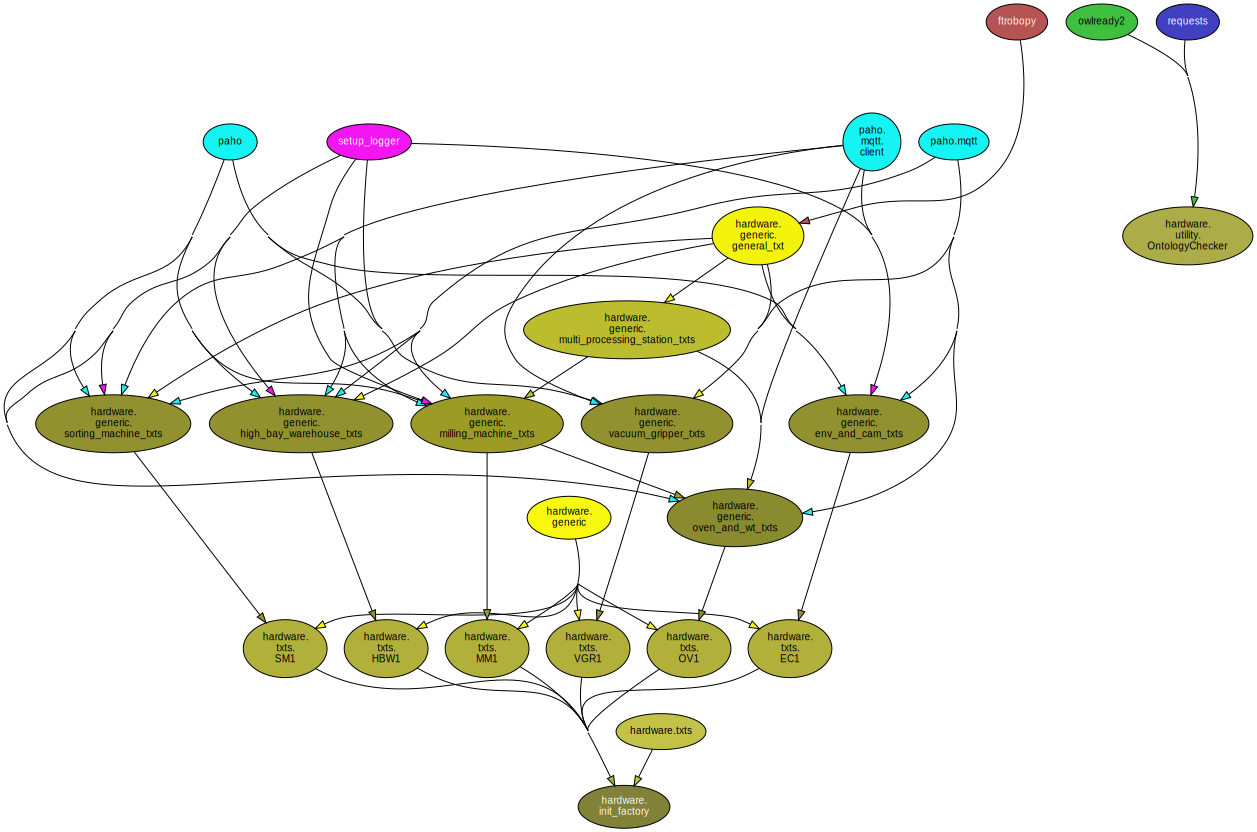
\includegraphics[width=\textwidth]{./assets/hardware}
    \caption{Dependency Graph}
    \label{dependencies}
    \label{fig:pre-refactor}
\end{figure}
A dependency graph in figure \ref{dependencies} is included to gain further knowledge on the coupling and cohesion of our software system. In particular, it depicts the dependencies within the classes of the hardware directory of the software system. By closer inspection, we observe one key characteristic of the modular structure. The characteristic being that most of the modules are related to individual stations, which indicate single responsibility associated to each station. There are no visible dependencies between the stations. This was visible in our analysis of code duplication, which showed that many functionalities are duplicated among the separate stations. As a consequence, having these characteristics, the code is argued to be low in coupling. This means that there are not many dependencies among the modules, which leads to the conclusion that \emph{Shotgun Surgery} should not be considered a code smell. This certainly a good indicator that refactoring towards microservices is feasible in this regard. 

Similarly, we can assume that given this modular structure, the software is also high in cohesion. In other words, the structure following this single responsibility principle suggests the code smell \emph{Divergent change} and \emph{Feature Envy} not to be an issue. Importantly, there should be a note of caution to these conclusions. Relying on looking at the modular structure to reach a conclusion about cohesion, does not suffice to disregard a code smell. Hence, the author can not provide a complete guarantee and only offers a prediction.

\section{Refactoring based on an Example}

We now turn to discussing how one would approach refactoring the code duplication within our software system. It has been mentioned in the beginning of the chapter that the volume of 24 duplicated blocks is in fact a duplication of 24 unique blocks. This means that each of these 24 duplications occurs multiple times within the code base. Both the amount of occurrences and block length, are crucial in determining which code duplications to start refactoring. The thesis will provide an overview of one particular code duplication, which has the largest block size and the maximum occurrence of six times. As may be presumed, each duplication is associated with one of the six stations. The particular duplication regards one method, which is responsible for setting the motor speed of the individual stations. Figure \ref{fig:pre-refactor} provides a better understanding of the underlying structure of the code duplication that needs to be refactored. 

\begin{figure}[htp]
    \centering
    \includegraphics[width=\textwidth]{./assets/board_extended}
    \caption{Code duplication Illustration (Before Refactoring)}
    \label{fig:pre-refactor}
\end{figure}

The six code duplicates can all be found in the web application of the software system. The content visualized for the particular method \emph{hbw\_set\_motor\_speed()}, is the same for the remaining five methods, indicated by the three dots. These methods are related both a queue mechanism and an RPC call that calls a station-specific method setting the motor speed. After carefully inspecting these methods, we arrive at the conclusion that these methods are code duplication themselves. Particularly, there exists a nested structure of code duplicates, in three hierarchical levels. In order to refactor our code duplication, we ought to also get rid of these nested duplications, as they are closely related to the method. 

Furthermore, by refactoring all of these methods, we will inevitably realize that these methods are not only used to set the motor speed. Namely, they are also contained at various location in the software system. Consequently, after unifying these methods, we can simplify code even more by transferring them to other locations. As an example, in addition to the method that sets the motor speed, there exists additional methods that \emph{get the motor speed} and \emph{reset the motor speed}. These all include the same methods that are responsible for the queue mechanism, which further provides  opportunities to simplify the code base of the software system. 

\begin{figure}[H]
    \centering
    \label{fig:simplified}
    \includegraphics[width=\textwidth]{./assets/board_simplified}
    \caption{Code duplciation Illustration (After Refactoring)}
\end{figure}

Figure \ref{fig:simplified} presents an overview of how the code is supposed to be structured after refactoring the code duplication. We immediately see that these changes result in a simpler structure, with much less code. In addition, using this example, we showed refactoring to be an activity that is dynamic. We have started with one unique code duplication, but ended with proposing various structural changes to improve the software system. The nested structure demonstrated the impact of the code smell to be much larger than anticipated. Hence, by refactoring one issue, we might discover another issue that is related to the previous issue. 